\chapter{Conception fonctionnelle et architecturale}

\section*{Introduction}
\addcontentsline{toc}{section}{Introduction}
Le chapitre précédent a défini le périmètre de JobTest et les besoins du recruteur. Le présent chapitre traduit ces besoins en une conception vérifiable dans l'application : responsabilités, données, interactions et déploiement logique. La conception sépare volontairement le calcul déterministe de correspondance de l'analyse générative. Ainsi, le recruteur conserve la décision finale ; le système restitue un résultat de correspondance et des éléments d'interprétation, sans automatiser l'embauche.

\section{Démarche de conception}
Dans le cycle en cascade retenu, la conception établit le passage des exigences du chapitre 2 vers des composants implémentables, avant leur réalisation et leur validation. Elle fixe les responsabilités et les échanges qui doivent demeurer stables lorsque l'interface ou l'infrastructure évoluent.

La notation UML 2.5.1 est employée de manière ciblée : le diagramme de classes représente les objets persistants et leurs liens, tandis que les diagrammes de séquence montrent l'ordre des appels et les alternatives importantes. La spécification UML de l'OMG sert de référence de notation \cite{omg_uml251}. Le diagramme global de cas d'utilisation reste celui de la figure~\ref{fig:uc-global}; il n'est donc pas reproduit ici.

\section{Vue fonctionnelle globale}
La vue complémentaire de la figure~\ref{fig:fonctionnelle} organise les fonctions par enchaînement plutôt que par acteur. L'authentification ouvre une session de recruteur. Celui-ci gère ses offres et ses candidats, lance l'évaluation puis consulte un résultat persistant. Le résultat constitue le point d'entrée du rapport PDF, de l'historique et de l'analyse approfondie. Cette dernière est une couche complémentaire : elle reçoit des informations déjà calculées et ne revient jamais modifier le score ni le verdict déterministe.

\begin{figure}[htbp]
\centering
\begin{tikzpicture}[node distance=8mm and 10mm]
  \node[archbox] (auth) {Authentification\\et session};
  \node[archbox,right=of auth] (jobs) {Offres d'emploi\\et candidats};
  \node[archbox,right=of jobs] (eval) {Évaluation\\hybride};
  \node[archbox,below=of eval] (result) {Résultat explicable\\persistant};
  \node[archbox,left=of result] (history) {Historique et\\consultation};
  \node[archbox,right=of result] (deep) {Analyse approfondie\\locale Ollama};
  \node[archbox,below=of result] (report) {Rapport PDF\\et téléchargement};
  \draw[-{Stealth[length=2mm]},line width=.5pt] (auth)--(jobs)--(eval)--(result);
  \draw[-{Stealth[length=2mm]},line width=.5pt] (result)--(history);
  \draw[-{Stealth[length=2mm]},line width=.5pt] (result)--(deep);
  \draw[-{Stealth[length=2mm]},line width=.5pt] (result)--(report);
  \draw[umlinclude] (deep.south west) to[bend right=20] node[below,font=\scriptsize,align=center]{contexte structuré ;\\aucun recalcul} (result.east);
\end{tikzpicture}

\caption{Vue de synthèse fonctionnelle de JobTest}
\label{fig:fonctionnelle}
\end{figure}

\section{Architecture logique de JobTest}
La solution déployée est un monolithe modulaire conteneurisé, et non un ensemble de microservices métier autonomes. Le navigateur ne joint publiquement que Nginx sur le port~80. Nginx relaie le préfixe \texttt{/api/v1/} vers FastAPI et les autres chemins vers Next.js. Les ports 3000, 8000, 5432 et 11434 sont internes au réseau Docker : ils ne sont pas publiés sur Internet.

La figure~\ref{fig:architecture-logique} représente cette organisation ainsi que les frontières réseau qui la délimitent.

\begin{figure}[htbp]
\centering
\begin{tikzpicture}[node distance=9mm and 11mm]
  \node[archbox,fill=green!7] (browser) {Navigateur\\recruteur};
  \node[archbox,right=of browser,fill=orange!10] (nginx) {Caddy (HTTPS)\\public :443};
  \node[archbox,right=of nginx] (web) {Next.js\\interne :3000};
  \node[archbox,below=18mm of web] (api) {FastAPI et services\\internes :8000};
  \node[archbox,below=18mm of nginx,minimum width=3.0cm] (layer1) {Layer 1 : TF--IDF,\\embeddings, compétences,\\décision et explication};
  \node[datastore,below=of layer1] (db) {PostgreSQL\\:5432};
  \node[archbox,below=of api] (ollama) {Ollama\\:11434};
  \draw[-{Stealth[length=2mm]},line width=.55pt] (browser)--node[above,font=\scriptsize]{HTTPS} (nginx);
  \draw[-{Stealth[length=2mm]},line width=.55pt] (nginx)--node[above,font=\scriptsize]{/} (web);
  \draw[-{Stealth[length=2mm]},line width=.55pt] (nginx.south) -- node[right,font=\scriptsize]{/api/v1} (api.west);
  \draw[-{Stealth[length=2mm]},line width=.55pt] (api.west)--(layer1.east);
  \draw[-{Stealth[length=2mm]},line width=.55pt] (api.south west)--(db.east);
  \draw[-{Stealth[length=2mm]},line width=.55pt] (api)--node[right,font=\scriptsize]{Layer 2} (ollama);
  \node[draw=black!55,dashed,rounded corners=2pt,fit=(web)(api)(db)(ollama)(layer1),inner sep=7mm,label={[font=\scriptsize]above:réseau Docker interne}] {};
\end{tikzpicture}

\caption{Architecture logique et frontières réseau de JobTest}
\label{fig:architecture-logique}
\end{figure}

La couche de présentation est une application Next.js. Son client API conserve le jeton bearer dans le stockage local du navigateur et utilise le même origin \texttt{/api/v1}. La couche FastAPI porte l'authentification, les routes HTTP, les contrôles d'appartenance et l'orchestration des services. Elle appelle en processus la Layer~1, composée des modèles TF--IDF, embeddings et compétences, du moteur de décision et du générateur d'explications.

La Layer~2 appelle Ollama à l'intérieur du réseau Docker avec un contexte structuré issu de l'évaluation déjà persistée. PostgreSQL est la persistance du déploiement; l'application conserve néanmoins SQLite comme valeur par défaut de développement à travers \texttt{DATABASE\_URL}. Le chapitre~6 détaillera les choix d'exploitation Azure, sans les confondre avec cette vue logique.

\section{Architecture applicative et responsabilités}
Le tableau~\ref{tab:modules-jobtest} relie les responsabilités de conception aux modules réellement présents. Les routes \texttt{/ui} sont un routeur de parité ajoutant une façade HTTP pour l'interface Next.js : elles réutilisent les mêmes services de calcul, modèles SQLAlchemy et moteur de décision.

{\scriptsize\setlength{\tabcolsep}{3pt}
\begin{longtable}{|>{\raggedright\arraybackslash}p{2.8cm}|>{\raggedright\arraybackslash}p{5.35cm}|>{\raggedright\arraybackslash}p{4.95cm}|}
\caption{Modules applicatifs et responsabilités}\label{tab:modules-jobtest}\\
\hline
\textbf{Couche ou module} & \textbf{Éléments vérifiés} & \textbf{Responsabilité}\\
\hline
\endfirsthead
\hline
\textbf{Couche ou module} & \textbf{Éléments vérifiés} & \textbf{Responsabilité}\\
\hline
\endhead
Interface utilisateur & \texttt{web/app}, composants d'analyse, \texttt{web/lib/api/client.ts} & Écrans Next.js, saisie des offres et CV, restitution des résultats, appel des routes et téléchargement du PDF.\\
\hline
Exposition HTTP & \texttt{src/api/routers/auth.py}, \texttt{src/api/routers/ui.py}, \texttt{src/api/main.py} & JWT, validation Pydantic, contrôle du recruteur connecté, routes métiers et transformation des réponses JSON.\\
\hline
Services métier & \texttt{src/matching/service.py}, \texttt{src/decisioning/decision\_engine.py} & Orchestration de l'évaluation, décision canonique, persistance atomique et métadonnées de reproductibilité.\\
\hline
Extraction et modèles & \texttt{src/parsing/parser.py}, \texttt{src/models}, \texttt{src/fusion/hybrid\_scorer.py} & Extraction de texte PDF/DOCX, scores TF--IDF, sémantique et compétences, puis agrégation hybride.\\
\hline
Explicabilité & \texttt{src/explainability/explainer.py} & Composantes de score, analyse des écarts, compétences et recommandations cohérentes avec le résultat déterministe.\\
\hline
Analyse approfondie & \texttt{src/ai/llm\_reasoning.py}, \texttt{DeepAnalysis.tsx} & Construction du contexte, appel Ollama local, validation JSON, contrôle de cohérence et restitution d'un état contrôlé.\\
\hline
Rapport PDF & \texttt{src/reporting/pdf\_generator.py}, \texttt{/report/pdf} & Composition ReportLab du rapport à partir du résultat, de l'explication et des recommandations déjà calculés.\\
\hline
Persistance & \texttt{src/models\_db.py}, \texttt{src/database.py} & Modèles SQLAlchemy, relations, transactions et adaptation SQLite/PostgreSQL par configuration.\\
\hline
\end{longtable}\par}
\normalsize

\section{Conception statique -- diagramme de classes global}
La figure~\ref{fig:classes-globales} privilégie les concepts métier et les attributs nécessaires à la compréhension. Les noms entre parenthèses correspondent aux classes techniques SQLAlchemy. Une analyse LLM n'est pas une table distincte : son enveloppe JSON est conservée dans \texttt{MatchResult.llm\_analysis\_json} uniquement lorsqu'elle est valide. De même, le rapport PDF est généré à la demande et ne possède pas d'entité persistée propre.

\begin{figure}[htbp]
\centering
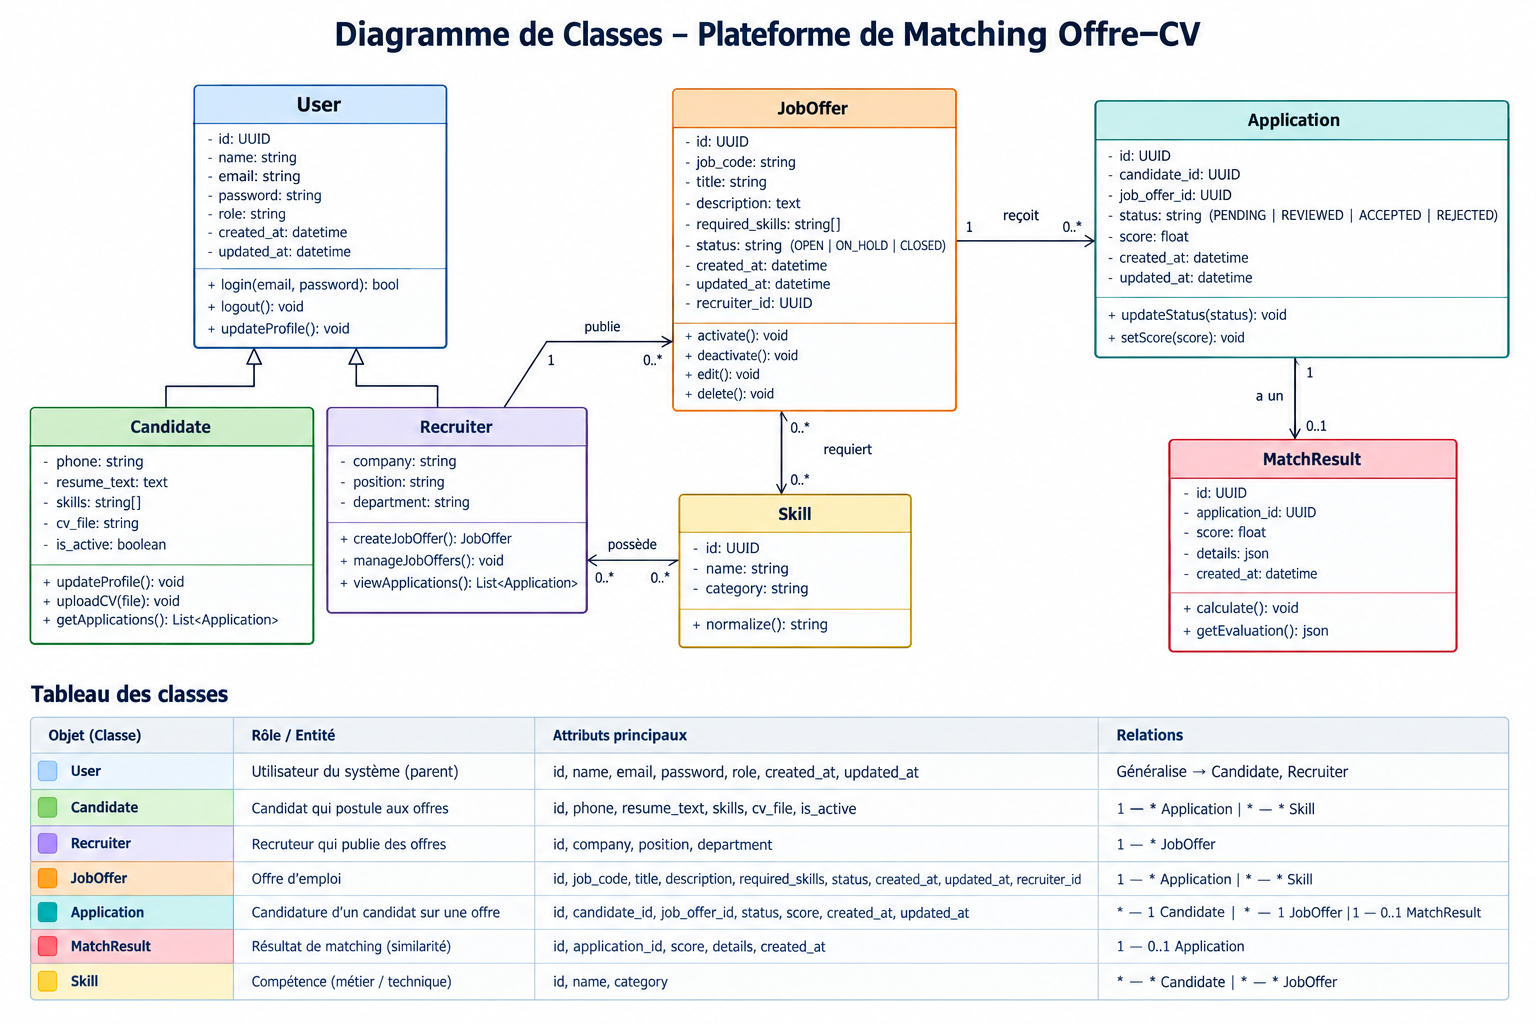
\includegraphics[width=.95\textwidth,height=.78\textheight,keepaspectratio]{img/diagrammes/classes.png}
\caption{Diagramme de classes métier simplifié de JobTest}
\label{fig:classes-globales}
\end{figure}

Un utilisateur recruteur possède des offres et des candidats. Un candidat peut regrouper plusieurs CV et plusieurs résultats de correspondance; chaque résultat se rattache au CV et à l'offre qui ont servi à son calcul. Les compétences sont normalisées dans \texttt{Skill} et reliées aux CV et aux offres par les tables d'association \texttt{cv\_skills} et \texttt{job\_skills}. Les chemins actuels d'évaluation conservent également le texte et les informations d'explication dans le résultat pour en permettre la consultation ultérieure.

\section{Conception dynamique -- diagrammes de séquence}

\subsection{Authentification du recruteur}
La connexion utilise le formulaire OAuth2 de FastAPI. Après vérification du mot de passe haché, l'API émet un JWT bearer. L'interface le stocke localement puis appelle \texttt{/auth/me} afin de charger le profil de session.

La figure~\ref{fig:seq-auth} détaille cet échange, depuis la soumission du formulaire jusqu'au chargement du profil.

\begin{figure}[htbp]
\centering
\begin{tikzpicture}[x=1cm,y=1cm]
  \node[seqpart] at (0,0) {Recruteur}; \node[seqpart] at (3.2,0) {Next.js};
  \node[seqpart] at (6.4,0) {FastAPI}; \node[seqpart] at (9.6,0) {Service\\d'authentification};
  \node[seqpart] at (12.8,0) {PostgreSQL};
  \foreach \x in {0,3.2,6.4,9.6,12.8} \draw[seqline] (\x,-.35)--(\x,-5.4);
  \draw[seqmsg] (0,-.8)--node[above]{identifiants} (3.2,-.8);
  \draw[seqmsg] (3.2,-1.35)--node[above]{POST /auth/login} (6.4,-1.35);
  \draw[seqmsg] (6.4,-1.9)--node[above]{vérifier mot de passe} (9.6,-1.9);
  \draw[seqmsg] (9.6,-2.45)--node[above]{rechercher e-mail} (12.8,-2.45);
  \draw[seqmsg] (12.8,-3.0)--node[above]{utilisateur} (9.6,-3.0);
  \draw[seqmsg] (9.6,-3.55)--node[above]{JWT bearer} (6.4,-3.55);
  \draw[seqmsg] (6.4,-4.1)--node[above]{jeton} (3.2,-4.1);
  \draw[seqmsg] (3.2,-4.65)--node[above]{GET /auth/me + bearer} (6.4,-4.65);
  \draw[seqmsg] (6.4,-5.15)--node[above]{profil de session} (3.2,-5.15);
\end{tikzpicture}

\caption{Séquence d'authentification du recruteur}
\label{fig:seq-auth}
\end{figure}

\subsection{Création d'une offre d'emploi}
L'écran des offres transmet le titre, la description, les compétences requises et l'état demandé. La route \texttt{/ui/job-offers} vérifie la présence du titre et de la description, associe l'offre au recruteur connecté et construit le code \texttt{JOB-AAAA-NNN} avant l'écriture en base.

La figure~\ref{fig:seq-offre} en retrace le déroulement.

\begin{figure}[htbp]
\centering
\begin{tikzpicture}[x=1cm,y=1cm]
  \node[seqpart] at (0,0) {Recruteur}; \node[seqpart] at (3.5,0) {Next.js};
  \node[seqpart] at (7,0) {FastAPI\\route /ui}; \node[seqpart] at (10.5,0) {PostgreSQL};
  \foreach \x in {0,3.5,7,10.5} \draw[seqline] (\x,-.35)--(\x,-5.0);
  \draw[seqmsg] (0,-.8)--node[above]{saisir offre} (3.5,-.8);
  \draw[seqmsg] (3.5,-1.4)--node[above]{POST /ui/job-offers} (7,-1.4);
  \draw[seqmsg] (7,-2.0)--node[above]{valider titre et description} (7.8,-2.0);
  \draw[seqmsg] (7,-2.6)--node[above]{compter les offres et générer\\JOB-AAAA-NNN} (10.5,-2.6);
  \draw[seqmsg] (7,-3.25)--node[above]{INSERT offre + recruteur\_id} (10.5,-3.25);
  \draw[seqmsg] (10.5,-3.85)--node[above]{offre créée} (7,-3.85);
  \draw[seqmsg] (7,-4.45)--node[above]{201 et offre sérialisée} (3.5,-4.45);
\end{tikzpicture}

\caption{Séquence de création d'une offre d'emploi}
\label{fig:seq-offre}
\end{figure}

\subsection{Évaluation d'un CV par rapport à une offre}
La figure~\ref{fig:seq-evaluation} représente le chemin canonique. Le CV est fourni comme texte ou par téléversement; dans ce dernier cas, le routeur extrait le texte du PDF ou du DOCX avant l'évaluation. L'offre doit appartenir au recruteur. Le service exécute les trois composantes, les agrège, applique les seuils et persiste un \texttt{MatchResult}.

Pour le modèle hybride par défaut, les scores élémentaires sont compris entre 0 et 1 et la formule effective est :
\[
S_h = 0{,}2S_{\mathrm{TF\text{-}IDF}} + 0{,}4S_{\mathrm{emb}} + 0{,}4S_{\mathrm{comp}}.
\]
Le pourcentage affiché vaut $100S_h$. Avec la configuration par défaut, le \texttt{DecisionEngine} produit \texttt{HIRE} si le score est supérieur ou égal à 75, \texttt{CONSIDER} s'il est compris entre 55 et strictement inférieur à 75, et \texttt{REJECT} en dessous de 55. Les seuils de session peuvent être transmis par l'interface, mais la configuration utilisée est enregistrée avec le résultat. Ce verdict est une recommandation algorithmique et non une décision de recrutement.

\begin{figure}[p]
\centering
\begin{tikzpicture}[x=1cm,y=1cm]
  \node[seqpart] at (0,0) {Recruteur}; \node[seqpart] at (2.7,0) {Next.js};
  \node[seqpart] at (5.4,0) {FastAPI}; \node[seqpart] at (8.1,0) {Service\\d'évaluation};
  \node[seqpart] at (10.8,0) {Layer 1}; \node[seqpart] at (13.5,0) {PostgreSQL};
  \foreach \x in {0,2.7,5.4,8.1,10.8,13.5} \draw[seqline] (\x,-.35)--(\x,-8.2);
  \draw[seqmsg] (0,-.8)--node[above]{choisir offre et CV} (2.7,-.8);
  \draw[seqmsg] (2.7,-1.35)--node[above]{POST /ui/evaluate\\ou /evaluate/file} (5.4,-1.35);
  \draw[seqmsg] (5.4,-1.9)--node[above]{valider CV et propriété de l'offre} (13.5,-1.9);
  \draw[seqmsg] (5.4,-2.5)--node[above]{texte normalisé + configuration} (8.1,-2.5);
  \draw[seqmsg] (8.1,-3.1)--node[above]{TF--IDF, embeddings,\\compétences} (10.8,-3.1);
  \draw[seqmsg] (10.8,-3.7)--node[above]{scores élémentaires} (8.1,-3.7);
  \draw[seqmsg] (8.1,-4.3)--node[above]{agréger 0,2 / 0,4 / 0,4} (10.8,-4.3);
  \draw[seqmsg] (10.8,-4.9)--node[above]{score hybride} (8.1,-4.9);
  \draw[seqmsg] (8.1,-5.5)--node[above]{décision, explication,\\recommandations} (10.8,-5.5);
  \draw[seqmsg] (8.1,-6.1)--node[above]{persist\_evaluation} (13.5,-6.1);
  \draw[seqmsg] (13.5,-6.7)--node[above]{MatchResult} (8.1,-6.7);
  \draw[seqmsg] (8.1,-7.3)--node[above]{résultat sérialisé} (5.4,-7.3);
  \draw[seqmsg] (5.4,-7.85)--node[above]{score, verdict, explication} (2.7,-7.85);
\end{tikzpicture}

\caption{Séquence centrale d'évaluation et de persistance d'un CV}
\label{fig:seq-evaluation}
\end{figure}
\clearpage

\subsection{Analyse approfondie avec Ollama}
Après le rendu de l'évaluation, le composant \texttt{DeepAnalysis} déclenche automatiquement un appel séparé pour l'identifiant du résultat; il peut aussi être relancé depuis l'interface. L'API reconstruit le contexte à partir du \texttt{MatchResult} sans recalculer la Layer~1. Ollama reçoit ce contexte structuré et doit fournir un JSON conforme. Une analyse réussie est ajoutée au résultat; sinon l'interface reçoit un état \texttt{disabled}, \texttt{unavailable}, \texttt{error} ou \texttt{inconsistent}. Dans tous les cas, le score et la décision de la Layer~1 restent inchangés.

L'enchaînement correspondant apparaît sur la figure~\ref{fig:seq-ollama}, où l'on voit que l'appel part d'un résultat déjà enregistré.

\begin{figure}[htbp]
\centering
\begin{tikzpicture}[x=1cm,y=1cm]
  \node[seqpart] at (0,0) {Next.js}; \node[seqpart] at (3.3,0) {FastAPI};
  \node[seqpart] at (6.6,0) {PostgreSQL}; \node[seqpart] at (9.9,0) {Service LLM};
  \node[seqpart] at (13.2,0) {Ollama local};
  \foreach \x in {0,3.3,6.6,9.9,13.2} \draw[seqline] (\x,-.35)--(\x,-6.5);
  \draw[seqmsg] (0,-.8)--node[above]{POST deep-analysis(match\_id)} (3.3,-.8);
  \draw[seqmsg] (3.3,-1.4)--node[above]{lire MatchResult possédé} (6.6,-1.4);
  \draw[seqmsg] (6.6,-2.0)--node[above]{scores, décision, explication} (3.3,-2.0);
  \draw[seqmsg] (3.3,-2.6)--node[above]{contexte structuré} (9.9,-2.6);
  \draw[seqmsg] (9.9,-3.2)--node[above]{/api/chat, format JSON} (13.2,-3.2);
  \draw[seqmsg] (13.2,-3.8)--node[above]{analyse JSON ou erreur} (9.9,-3.8);
  \draw[dashed,rounded corners=1pt] (2.5,-4.25) rectangle (10.7,-5.2);
  \node[anchor=west,font=\scriptsize] at (2.6,-4.42) {\textit{alt} statut \texttt{ok}};
  \draw[seqmsg] (9.9,-4.75)--node[above]{enveloppe valide} (3.3,-4.75);
  \draw[seqmsg] (3.3,-5.0)--node[below]{persister llm\_analysis\_json} (6.6,-5.0);
  \draw[seqmsg] (3.3,-5.75)--node[above]{statut contrôlé} (0,-5.75);
  \node[align=left,font=\scriptsize,anchor=west] at (.1,-6.35) {\textit{Sinon : disabled, unavailable, error ou inconsistent ; score et verdict inchangés.}};
\end{tikzpicture}

\caption{Séquence d'analyse approfondie, additive à la Layer~1}
\label{fig:seq-ollama}
\end{figure}

\subsection{Génération du rapport PDF}
Le téléchargement demande au serveur un document à partir du résultat, de l'explication et des recommandations déjà affichés. FastAPI délègue la mise en page au générateur ReportLab et retourne les octets PDF avec une en-tête de pièce jointe. Cette opération ne crée pas de nouvelle évaluation et ne modifie pas le résultat de correspondance.

La figure~\ref{fig:seq-pdf} montre la séquence suivie jusqu'au téléchargement du document.

\begin{figure}[htbp]
\centering
\begin{tikzpicture}[x=1cm,y=1cm]
  \node[seqpart] at (0,0) {Recruteur}; \node[seqpart] at (3.5,0) {Next.js};
  \node[seqpart] at (7,0) {FastAPI}; \node[seqpart] at (10.5,0) {Générateur\\ReportLab};
  \foreach \x in {0,3.5,7,10.5} \draw[seqline] (\x,-.35)--(\x,-4.7);
  \draw[seqmsg] (0,-.8)--node[above]{exporter le rapport} (3.5,-.8);
  \draw[seqmsg] (3.5,-1.45)--node[above]{POST /report/pdf\\résultat + explication} (7,-1.45);
  \draw[seqmsg] (7,-2.1)--node[above]{composer le document} (10.5,-2.1);
  \draw[seqmsg] (10.5,-2.75)--node[above]{octets PDF} (7,-2.75);
  \draw[seqmsg] (7,-3.4)--node[above]{application/pdf + pièce jointe} (3.5,-3.4);
  \draw[seqmsg] (3.5,-4.05)--node[above]{téléchargement} (0,-4.05);
\end{tikzpicture}

\caption{Séquence de génération et téléchargement d'un rapport PDF}
\label{fig:seq-pdf}
\end{figure}

\section{Conception des données}
Le modèle relationnel est porté par SQLAlchemy. \texttt{users.email}, \texttt{skills.name} et \texttt{job\_offers.job\_code} sont déclarés uniques. Les clés étrangères relient candidats et offres au recruteur, les CV aux candidats, puis les résultats à leur candidat, CV et offre. Les suppressions en cascade sont configurées entre candidat et CV, ainsi qu'entre candidat ou offre et résultats de correspondance.

Le résultat de correspondance est l'élément de traçabilité principal : il conserve les scores hybride, sémantique, lexical et compétences, la décision, les seuils utilisés, la version du modèle, la méthode et les poids. L'explication et les recommandations sont sérialisées dans \texttt{explanation\_json}; l'analyse approfondie valide est ajoutée dans \texttt{llm\_analysis\_json}. Les comparaisons de modèles et le benchmark de qualité ne créent pas de résultats persistants.

En développement, la valeur par défaut de \texttt{DATABASE\_URL} pointe vers SQLite et l'application active les clés étrangères SQLite. Dans le déploiement conteneurisé, cette variable cible PostgreSQL~16. Les mêmes modèles SQLAlchemy sont employés; la différence porte sur le moteur de base de données, non sur le modèle métier présenté.

\section{Principes de conception retenus}
\begin{itemize}
  \item \textbf{Séparation des responsabilités :} Next.js présente et collecte, FastAPI orchestre, les services calculent, SQLAlchemy persiste et Ollama interprète qualitativement.
  \item \textbf{Traçabilité et reproductibilité :} le résultat conserve les composantes, poids, version, méthode et seuils actifs lors de son calcul.
  \item \textbf{Isolation :} la pile Docker place PostgreSQL, FastAPI, Next.js et Ollama sur un réseau interne; seul Nginx expose le port~80.
  \item \textbf{Dégradation contrôlée :} l'indisponibilité, l'erreur ou l'incohérence de la Layer~2 est représentée par un état explicite, sans bloquer l'évaluation déterministe.
  \item \textbf{Responsabilité humaine :} la décision \texttt{HIRE}/\texttt{CONSIDER}/\texttt{REJECT} facilite l'examen d'un dossier; le recruteur demeure responsable de la décision finale.
\end{itemize}

\section*{Conclusion}
\addcontentsline{toc}{section}{Conclusion}
La conception de JobTest articule une interface Next.js, une API FastAPI, une persistance relationnelle et deux couches d'intelligence aux rôles distincts. Les diagrammes ont montré la conservation d'un résultat traçable, depuis l'authentification jusqu'au rapport et à l'analyse approfondie. Le chapitre suivant détaillera la conception et l'évaluation du moteur intelligent, notamment ses composantes de correspondance et ses résultats de validation.
